% Sandia National Laboratories is a multimission laboratory managed and
% operated by National Technology & Engineering Solutions of Sandia, LLC, a
% wholly owned subsidiary of Honeywell International Inc., for the U.S.
% Department of Energy’s National Nuclear Security Administration under
% contract DE-NA0003525.

% Copyright 2002-2020 National Technology & Engineering Solutions of Sandia,
% LLC (NTESS).


\begin{Device}\label{Z_DEVICE}

\symbol
{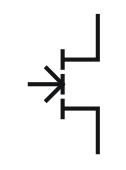
\includegraphics{nmesfetSymbol}}
{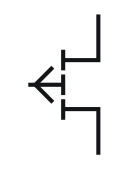
\includegraphics{pmesfetSymbol}}

\device
\begin{alltt}
Z<name> < drain node> <gate node> <source node> <model name>
+ [area value] [device parameters]
\end{alltt}

\model
\begin{alltt}
.MODEL <model name> NMF [model parameters]
.MODEL <model name> PMF [model parameters]
\end{alltt}

\examples
\begin{alltt}
Z1 2 3 0 MESMOD AREA=1.4
Z1 7 2 3 ZM1
\end{alltt}

\parameters

\begin{Parameters}

\param{drain node}
Node connected to drain.

\param{gate node}
Node connected to gate.

\param{source node}
Node connected to source.

\param{source node}
Name of model defined in .MODEL line.

\param{area value}

The \texttt{MESFET} is modeled as an intrinsic FET using an ohmic
resistance (\texttt{RD/area}) in series with the drain and another ohmic
resistance (\texttt{RS/area}) in series with the source.  \texttt{area value}
is a scaling factor with a default of 1.

\param{device parameters}

Parameters listed in Table~\ref{Z_1_Device_Instance_Params} may be
provided as space separated \texttt{<parameter>=<value>} specifications
as needed.  Any number of parameters may be specified.

\end{Parameters}

\comments

Although MESFETs can be made of Si, such devices are not as common as
GaAs MESFETS.  And since the mobility of electrons is much higher than
holes in GaAs, nearly all commercial devices are n-type MESFETS.

\end{Device}

\pagebreak

\paragraph{Device Parameters}
% This table was generated by Xyce:
%   Xyce -doc Z 1
%
\index{mesfet!device instance parameters}
\begin{DeviceParamTableGenerated}{MESFET Device Instance Parameters}{Z_1_Device_Instance_Params}
AREA & device area & m$^{2}$ & 1 \\ \hline
TEMP & Device temperature & -- & Ambient Temperature \\ \hline
\end{DeviceParamTableGenerated}


\paragraph{Model Parameters}
% This table was generated by Xyce:
%   Xyce -doc Z 1
%
\index{mesfet!device model parameters}
\begin{DeviceParamTableGenerated}{MESFET Device Model Parameters}{Z_1_Device_Model_Params}
AF & Flicker noise exponent & -- & 1 \\ \hline
ALPHA & Saturation voltage parameter & V$^{-1}$ & 2 \\ \hline
B & Doping tail parameter & V$^{-1}$ & 0.3 \\ \hline
BETA & Transconductance parameter & A/V$^{2}$ & 0.0025 \\ \hline
CGD & Zero-bias gate-drain junction capacitance & F & 0 \\ \hline
CGS & Zero-bias gate-source junction capacitance & F & 0 \\ \hline
FC & Coefficient for forward-bias depletion capacitance & F & 0.5 \\ \hline
IS & Gate junction saturation current & A & 1e-14 \\ \hline
KF & Flicker noise coefficient & -- & 0.05 \\ \hline
LAMBDA & Channel length modulation & V$^{-1}$ & 0 \\ \hline
PB & Gate junction potential & V & 1 \\ \hline
RD & Drain ohmic resistance & $\mathsf{\Omega}$ & 0 \\ \hline
RS & Source ohmic resistance & $\mathsf{\Omega}$ & 0 \\ \hline
TEMPMODEL & Specifies the type of parameter interpolation over temperature & -- & 'NONE' \\ \hline
TNOM & Nominal device temperature & $^\circ$C & Ambient Temperature \\ \hline
VTO & Threshold voltage & V & 0 \\ \hline
\end{DeviceParamTableGenerated}


\paragraph{MESFET Power Calculations}
Power dissipated in the transistor is calculated with $I_{D}*V_{DS}+I_{G}*V_{GS}$ where
$I_{D}$ is the drain current, $I_{G}$ is the gate current, $V_{DS}$ is the 
voltage drop between the drain and the source and $V_{GS}$ is the voltage drop 
between the gate and the source. This formula may differ from other simulators,
such as HSPICE and PSpice.
